\documentclass[a4paper,10pt,twocolumn]{ltjarticle}
\usepackage{kaitoushu}

% グラフ用の共通スタイル定義
\pgfplotsset{
  myaxis/.style={
    axis lines=middle,
    xlabel={$x$}, ylabel={$y$},
    every axis x label/.style={at={(ticklabel* cs:1)},anchor=west},
    every axis y label/.style={at={(ticklabel* cs:1)},anchor=south},
    tick label style={font=\scriptsize},
    label style={font=\small},
    width=5.5cm, height=5cm,
    grid=none,
    samples=100,
  }
}

\begin{document}

\problemrange{4章：指数関数と対数関数（201--247）}

%=============================================================
% Basic (p.44) 指数
%=============================================================

\mondai{201}{次の値を根号を用いて表せ．}
\kotae{
$n$ 乗根の定義：$a$ の $n$ 乗根とは，$n$ 乗すると $a$ になる数．$\sqrt[n]{a}$ で表す．

(1) 6の3乗根：$\sqrt[3]{6}$

(2) 10の4乗根：$\sqrt[4]{10}$

(3) $-12$の5乗根：$\sqrt[5]{-12}$

（奇数乗根は負の数にも存在する）
}

\mondai{202}{次の式を簡単にせよ．}
\kotae{
根号の計算では，$\sqrt[n]{a^{m}}=a^{m/n}$ を利用する．

(1) $\sqrt{2}\sqrt{32}=\sqrt{2\cdot32}=\sqrt{64}=8$

(2) $(\sqrt[3]{5})^{4}\sqrt[3]{25}=5^{4/3}\cdot5^{2/3}=5^{(4+2)/3}=5^{2}=25$

(3) $\sqrt[3]{27}\sqrt[3]{3}=\sqrt[3]{27\cdot3}=\sqrt[3]{81}=\sqrt[3]{3^{4}}=3\sqrt[3]{3}$

(4) $\dfrac{\sqrt[3]{48}}{\sqrt[3]{6}}=\sqrt[3]{\dfrac{48}{6}}=\sqrt[3]{8}=2$
}

\mondai{203}{次の計算をせよ．ただし，$a\neq0$，$b\neq0$ とする．}
\kotae{
指数法則：$a^{m}\cdot a^{n}=a^{m+n}$，$(a^{m})^{n}=a^{mn}$，$(ab)^{n}=a^{n}b^{n}$．

(1) $3^{8}\times\left(\dfrac{1}{9}\right)^{3}=3^{8}\times(3^{-2})^{3}=3^{8}\times3^{-6}=3^{2}=9$

(2) $10^{2}\times5^{-3}\times\left(\dfrac{1}{4}\right)^{-1}=10^{2}\times5^{-3}\times4$

$=\dfrac{100\times4}{125}=\dfrac{400}{125}=\dfrac{16}{5}$

(3) $(ab^{3})^{2}\times(a^{-1}b^{2})^{-1}=a^{2}b^{6}\times a\,b^{-2}=a^{3}b^{4}$

(4) $\dfrac{(9ab^{-2})^{2}}{(3a^{-2}b^{2})^{3}}=\dfrac{81a^{2}b^{-4}}{27a^{-6}b^{6}}=\dfrac{81}{27}\cdot a^{2-(-6)}\cdot b^{-4-6}=3a^{8}b^{-10}=\dfrac{3a^{8}}{b^{10}}$
}

\mondai{204}{次の (1), (2) については $a^{m/n}$ の形に，(3), (4) については根号を用いて表せ．ただし，$a>0$ とする．}
\kotae{
変換公式：$\sqrt[n]{a^{m}}=a^{m/n}$

(1) $\sqrt{a^{5}}=a^{5/2}$

(2) $\dfrac{1}{\sqrt[3]{a^{3}}}=a^{-3/3}=a^{-1}$

（別解：$\dfrac{1}{\sqrt[3]{a^3}}=\dfrac{1}{a}=a^{-1}$）

(3) $a^{2/5}=\sqrt[5]{a^{2}}$

(4) $a^{-1/2}=\dfrac{1}{a^{1/2}}=\dfrac{1}{\sqrt{a}}$
}

\mondai{205}{$a>0$ のとき，次の式を計算せよ．}
\kotae{
有理数指数の計算も指数法則がそのまま使える．

(1) $(a^{-1/2})^{4/3}=a^{(-1/2)\cdot(4/3)}=a^{-2/3}$

(2) $\dfrac{a^{1/2}}{a^{-1/4}}=a^{1/2-(-1/4)}=a^{1/2+1/4}=a^{3/4}$

(3) $a^{1.2}\times a^{0.4}=a^{1.2+0.4}=a^{1.6}=a^{8/5}$
}

\mondai{206}{指数法則を用いて，次の式を計算せよ．ただし，$a>0$ とする．}
\kotae{
根号を指数に直してから計算する．

(1) $\sqrt[4]{a^{2}}\times\sqrt[4]{a^{3}}=a^{2/4}\cdot a^{3/4}=a^{5/4}=\sqrt[4]{a^{5}}=a\sqrt[4]{a}$

(2) $\dfrac{a\sqrt[4]{a}}{\sqrt{a}}=\dfrac{a\cdot a^{1/4}}{a^{1/2}}=a^{1+1/4-1/2}=a^{3/4}=\sqrt[4]{a^{3}}$

(3) $\sqrt[3]{\sqrt[3]{a}}=\sqrt[3]{a^{1/3}}=(a^{1/3})^{1/3}=a^{1/9}=\sqrt[9]{a}$
}

\mondai{207}{次の関数のグラフをかけ．}
\kotae{
指数関数 $y=a^{x}$ の基本的性質：$a>1$ なら右上がり，$0<a<1$ なら右下がり．
必ず点$(0,1)$を通る．

(1) $y=4^{x}$

\begin{tikzpicture}
\begin{axis}[myaxis, xmin=-3,xmax=3,ymin=-0.5,ymax=6,
  ytick={1,2,3,4,5}]
\addplot[thick,blue,domain=-2.5:1.3]{4^x};
\addplot[only marks,mark=*,mark size=1.5pt] coordinates {(0,1)};
\node[font=\scriptsize,above left] at (axis cs:0,1) {$(0,1)$};
\end{axis}
\end{tikzpicture}

(2) $y=4^{x-1}$

$y=4^{x}$ を$x$方向に1平行移動．点$(1,1)$を通る．

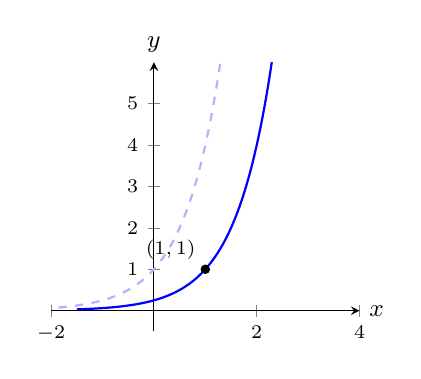
\begin{tikzpicture}
\begin{axis}[myaxis, xmin=-2,xmax=4,ymin=-0.5,ymax=6,
  ytick={1,2,3,4,5}]
\addplot[thick,blue,domain=-1.5:2.3]{4^(x-1)};
\addplot[thick,blue!30,dashed,domain=-2.5:1.3]{4^x};
\addplot[only marks,mark=*,mark size=1.5pt] coordinates {(1,1)};
\node[font=\scriptsize,above left] at (axis cs:1,1) {$(1,1)$};
\end{axis}
\end{tikzpicture}

(3) $y=\left(\dfrac{1}{4}\right)^{x}=4^{-x}$

$y=4^{x}$ の$y$軸対称．右下がり．

\begin{tikzpicture}
\begin{axis}[myaxis, xmin=-3,xmax=3,ymin=-0.5,ymax=6,
  ytick={1,2,3,4,5}]
\addplot[thick,blue,domain=-1.3:2.5]{4^(-x)};
\addplot[only marks,mark=*,mark size=1.5pt] coordinates {(0,1)};
\node[font=\scriptsize,above right] at (axis cs:0,1) {$(0,1)$};
\end{axis}
\end{tikzpicture}
}

\mondai{208}{グラフの対称移動の公式を用いて，次の関数のグラフをかけ．}
\kotae{
(1) $y=-4^{x}$：$y=4^{x}$ の$x$軸対称（$y\to-y$）

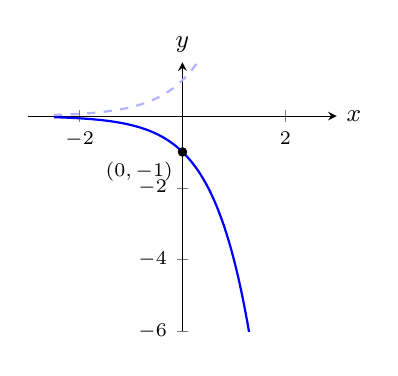
\begin{tikzpicture}
\begin{axis}[myaxis, xmin=-3,xmax=3,ymin=-6,ymax=1.5]
\addplot[thick,blue!30,dashed,domain=-2.5:1.3]{4^x};
\addplot[thick,blue,domain=-2.5:1.3]{-4^x};
\addplot[only marks,mark=*,mark size=1.5pt] coordinates {(0,-1)};
\node[font=\scriptsize,below left] at (axis cs:0,-1) {$(0,-1)$};
\end{axis}
\end{tikzpicture}

(2) $y=-4^{-x}$：$y=4^{x}$ の原点対称（$x\to-x$，$y\to-y$）

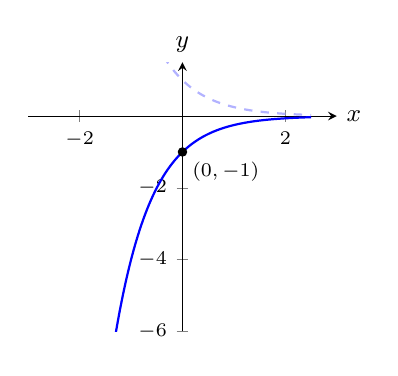
\begin{tikzpicture}
\begin{axis}[myaxis, xmin=-3,xmax=3,ymin=-6,ymax=1.5]
\addplot[thick,blue!30,dashed,domain=-1.3:2.5]{4^(-x)};
\addplot[thick,blue,domain=-1.3:2.5]{-4^(-x)};
\addplot[only marks,mark=*,mark size=1.5pt] coordinates {(0,-1)};
\node[font=\scriptsize,below right] at (axis cs:0,-1) {$(0,-1)$};
\end{axis}
\end{tikzpicture}
}

\mondai{209}{次の方程式を解け．}
\kotae{
指数方程式は，両辺の底をそろえて指数を比較する．

(1) $2^{2x}=2\sqrt[3]{2}=2^{1}\cdot2^{1/3}=2^{4/3}$

$2x=\dfrac{4}{3}$ → $x=\dfrac{2}{3}$

(2) $3^{-x+1}=\sqrt{243}=\sqrt{3^{5}}=3^{5/2}$

$-x+1=\dfrac{5}{2}$，$x=1-\dfrac{5}{2}=-\dfrac{3}{2}$

(3) $9^{x}-7\cdot3^{x}-18=0$

$3^{x}=t$ とおくと $t^{2}-7t-18=0$（$9^{x}=(3^{x})^{2}=t^{2}$）

$(t-9)(t+2)=0$．$t>0$ より $t=9$

$3^{x}=9=3^{2}$ → $x=2$
}

\mondai{210}{次の不等式を解け．}
\kotae{
底が1より大きい指数関数は単調増加なので，不等号の向きが保たれる．

(1) $8^{x}>16$

$(2^{3})^{x}>2^{4}$，$2^{3x}>2^{4}$

底 $2>1$ より $3x>4$ → $x>\dfrac{4}{3}$

(2) $\left(\dfrac{1}{5}\right)^{x+3}<\dfrac{1}{25}$

$5^{-(x+3)}<5^{-2}$

底 $5>1$ なので $-(x+3)<-2$，$-x-3<-2$，$-x<1$ → $x>-1$
}

%=============================================================
% Check (p.45) 指数
%=============================================================

\mondai{211}{次の式を簡単にせよ．}
\kotae{
(1) $\sqrt[3]{-8}\sqrt[5]{-243}=(-2)\cdot(-3)=6$

(2) $\sqrt[4]{(-2)^{4}}\sqrt[3]{125}=|-2|\cdot5=2\cdot5=10$

（偶数乗根は絶対値になることに注意）

(3) $(\sqrt[3]{2})^{5}\sqrt[3]{54}=2^{5/3}\cdot(2\cdot27)^{1/3}=2^{5/3}\cdot2^{1/3}\cdot3=2^{2}\cdot3=12$

(4) $\dfrac{\sqrt[3]{24}}{(\sqrt[5]{18})^{3}}$

$=\dfrac{(24)^{1/3}}{(18)^{3/5}}=\dfrac{(2^{3}\cdot3)^{1/3}}{(2\cdot3^{2})^{3/5}}=\dfrac{2\cdot3^{1/3}}{2^{3/5}\cdot3^{6/5}}=2^{2/5}\cdot3^{1/3-6/5}=2^{2/5}\cdot3^{-13/15}$

$=\dfrac{2^{2/5}}{3^{13/15}}=\dfrac{\sqrt[5]{4}}{\sqrt[15]{3^{13}}}$
}

\mondai{212}{次の式を $a^{p}$ の形に表せ．ただし，$a>0$ とする．}
\kotae{
(1) $a\sqrt[3]{a}=a^{1}\cdot a^{1/3}=a^{4/3}$

(2) $\sqrt{\sqrt[3]{a^{2}}}=\sqrt{a^{2/3}}=(a^{2/3})^{1/2}=a^{1/3}$

(3) $\dfrac{1}{a^{2}\sqrt[4]{a^{3}}}=\dfrac{1}{a^{2}\cdot a^{3/4}}=a^{-(2+3/4)}=a^{-11/4}$

(4) $\dfrac{a^{2}}{\sqrt[5]{\sqrt[6]{a}}}=\dfrac{a^{2}}{(a^{1/6})^{1/5}}=\dfrac{a^{2}}{a^{1/30}}=a^{2-1/30}=a^{59/30}$
}

\mondai{213}{次の式を，根号を用いて表せ．ただし，$a>0$ とする．}
\kotae{
(1) $a^{1/2}\times a^{1/3}=a^{1/2+1/3}=a^{5/6}=\sqrt[6]{a^{5}}$

(2) $\dfrac{a^{5/4}}{a^{3/2}}=a^{5/4-3/2}=a^{-1/4}=\dfrac{1}{\sqrt[4]{a}}$
}

\mondai{214}{次の計算せよ．ただし，$a>0$ とする．}
\kotae{
(1) $(2a^{2})^{2/3}\times(2a^{-1})^{1/3}=2^{2/3}a^{4/3}\times2^{1/3}a^{-1/3}=2^{1}\cdot a^{1}=2a$

(2) $(a^{1/2}+a^{-1/2})^{2}=a+2+a^{-1}=a+2+\dfrac{1}{a}$

（展開公式 $(p+q)^{2}=p^{2}+2pq+q^{2}$ で $pq=a^{1/2}\cdot a^{-1/2}=1$）

(3) $\dfrac{\sqrt[3]{a^{2}}\times\sqrt{a}}{\sqrt[6]{a^{5}}}=\dfrac{a^{2/3}\cdot a^{1/2}}{a^{5/6}}=a^{2/3+1/2-5/6}=a^{4/6+3/6-5/6}=a^{2/6}=a^{1/3}=\sqrt[3]{a}$

(4) $\left(\dfrac{\sqrt[4]{a}}{\sqrt[3]{a}}\right)^{2}\times\sqrt[6]{a}=\left(\dfrac{a^{1/4}}{a^{1/3}}\right)^{2}\times a^{1/6}=(a^{-1/12})^{2}\times a^{1/6}=a^{-1/6}\times a^{1/6}=a^{0}=1$
}

\mondai{215}{次の関数のグラフは $y=3^{x}$ のグラフをどのように移動したものか．}
\kotae{
(1) $y=3^{x}+1$：$y$軸方向に$1$平行移動（上に1ずらす）

(2) $y=-3^{-x}$：まず$y$軸対称（$x\to-x$で$y=3^{-x}$），次に$x$軸対称（$y\to-y$）

つまり原点に関して対称移動．
}

\mondai{216}{次の方程式を解け．}
\kotae{
(1) $4^{x}-7\cdot2^{x}-8=0$

$2^{x}=t>0$ とおく．$t^{2}-7t-8=0$，$(t-8)(t+1)=0$

$t>0$ より $t=8$．$2^{x}=8=2^{3}$ → $x=3$

(2) $2\left(\dfrac{1}{4}\right)^{x}-9\left(\dfrac{1}{2}\right)^{x}+4=0$

$\left(\dfrac{1}{2}\right)^{x}=t>0$ とおく．$\left(\dfrac{1}{4}\right)^{x}=t^{2}$

$2t^{2}-9t+4=0$，$(2t-1)(t-4)=0$

$t=\dfrac{1}{2}$ または $t=4$

$\left(\dfrac{1}{2}\right)^{x}=\dfrac{1}{2}=\left(\dfrac{1}{2}\right)^{1}$ → $x=1$

$\left(\dfrac{1}{2}\right)^{x}=4=\left(\dfrac{1}{2}\right)^{-2}$ → $x=-2$
}

\mondai{217}{次の不等式を解け．}
\kotae{
(1) $3^{2x-1}<\dfrac{1}{\sqrt[4]{81}}=\dfrac{1}{81^{1/4}}=\dfrac{1}{3}=3^{-1}$

底 $3>1$ より $2x-1<-1$，$2x<0$ → $x<0$

(2) $\left(\dfrac{1}{2}\right)^{x}<\sqrt[3]{32}=2^{5/3}$

$2^{-x}<2^{5/3}$．底 $2>1$ より $-x<\dfrac{5}{3}$ → $x>-\dfrac{5}{3}$
}

%=============================================================
% Basic (p.49) 対数
%=============================================================

\mondai{225}{次の値を求めよ．}
\kotae{
対数の定義：$\log_{a}b=c$ $\Leftrightarrow$ $a^{c}=b$．「$a$ を何乗すると $b$ になるか」．

(1) $\log_{5}25=\log_{5}5^{2}=2$

(2) $\log_{3}\dfrac{1}{27}=\log_{3}3^{-3}=-3$

(3) $\log_{0.1}0.001=\log_{0.1}(0.1)^{3}=3$

(4) $\log_{4}1=0$\quad（任意の底で $\log_{a}1=0$）

(5) $\log_{2}0.25=\log_{2}\dfrac{1}{4}=\log_{2}2^{-2}=-2$

(6) $\log_{2}\sqrt[5]{8}=\log_{2}(2^{3})^{1/5}=\log_{2}2^{3/5}=\dfrac{3}{5}$
}

\mondai{226}{次の式を計算せよ．}
\kotae{
対数の性質：$\log_{a}MN=\log_{a}M+\log_{a}N$，$\log_{a}\dfrac{M}{N}=\log_{a}M-\log_{a}N$，$\log_{a}M^{k}=k\log_{a}M$．

(1) $\log_{2}64=\log_{2}2^{6}=6$

(2) $\log_{3}6+\log_{3}\dfrac{3}{2}=\log_{3}\!\left(6\cdot\dfrac{3}{2}\right)=\log_{3}9=2$

(3) $\log_{5}2-\log_{5}10=\log_{5}\dfrac{2}{10}=\log_{5}\dfrac{1}{5}=\log_{5}5^{-1}=-1$

(4) $\dfrac{1}{2}\log_{2}10+\log_{2}\dfrac{4}{\sqrt{5}}$

$=\log_{2}\sqrt{10}+\log_{2}\dfrac{4}{\sqrt{5}}=\log_{2}\!\left(\sqrt{10}\cdot\dfrac{4}{\sqrt{5}}\right)=\log_{2}(4\sqrt{2})=\log_{2}2^{5/2}=\dfrac{5}{2}$
}

\mondai{227}{等式 $\log_{a}\dfrac{1}{\sqrt[n]{M}}=-\dfrac{1}{n}\log_{a}M$ を証明せよ．}
\kotae{
左辺$=\log_{a}M^{-1/n}=-\dfrac{1}{n}\log_{a}M=$右辺

（$\log_{a}M^{k}=k\log_{a}M$ を使った）\qed
}

\mondai{228}{$A,B,C,a$ は正の数で $a\neq1$ とするとき，次の問いに答えよ．}
\kotae{
(1) $\log_{a}\dfrac{A}{B}+\log_{a}\dfrac{B}{C}+\log_{a}\dfrac{C}{A}=0$ を証明．

左辺$=\log_{a}\!\left(\dfrac{A}{B}\cdot\dfrac{B}{C}\cdot\dfrac{C}{A}\right)=\log_{a}1=0=$右辺 \qed

(2) $\log_{3}\sqrt{6}+\log_{3}\sqrt{10}-\log_{3}\sqrt{20}$

$=\log_{3}\dfrac{\sqrt{6}\cdot\sqrt{10}}{\sqrt{20}}=\log_{3}\sqrt{\dfrac{60}{20}}=\log_{3}\sqrt{3}=\dfrac{1}{2}$
}

\mondai{229}{$\log_{a}2$ の値を求めよ．}
\kotae{
問題文から底 $a$ が指定されていない場合，底の変換公式等を利用する．

※ この問題は教科書 p.115 を参照．底が $10$ の場合：$\log_{10}2\approx0.3010$（常用対数）．
}

\mondai{230}{1でない正の数 $a,b,c$ について，次の式を計算せよ．$(\log_{a}b)\cdot(\log_{b}c)\cdot(\log_{c}a)$}
\kotae{
底の変換公式：$\log_{a}b=\dfrac{\log b}{\log a}$（底は何でもよい）

$(\log_{a}b)(\log_{b}c)(\log_{c}a)=\dfrac{\log b}{\log a}\cdot\dfrac{\log c}{\log b}\cdot\dfrac{\log a}{\log c}=1$

（分子と分母がすべて約分される）
}

\mondai{231}{次の式を簡単にせよ．}
\kotae{
底の変換公式で底をそろえてから計算する．

(1) $(\log_{2}27)\cdot(\log_{9}8)$

$=\log_{2}3^{3}\cdot\log_{9}2^{3}=3\log_{2}3\cdot3\log_{9}2=9\log_{2}3\cdot\dfrac{\log 2}{\log 9}$

$=9\cdot\dfrac{\log 3}{\log 2}\cdot\dfrac{\log 2}{2\log 3}=9\cdot\dfrac{1}{2}=\dfrac{9}{2}$

(2) $(\log_{3}125)\cdot(\log_{4}3)\cdot(\log_{5}32)$

$=\dfrac{\log 125}{\log 3}\cdot\dfrac{\log 3}{\log 4}\cdot\dfrac{\log 32}{\log 5}=\dfrac{3\log 5}{\log 3}\cdot\dfrac{\log 3}{2\log 2}\cdot\dfrac{5\log 2}{\log 5}=\dfrac{3\cdot5}{2}=\dfrac{15}{2}$
}

\mondai{232}{次の関数のグラフをかけ．}
\kotae{
対数関数 $y=\log_{a}x$ の基本性質：必ず点$(1,0)$を通り，$a>1$ なら右上がり，$0<a<1$ なら右下がり．

(1) $y=\log_{3}x$

\begin{tikzpicture}
\begin{axis}[myaxis, xmin=-1,xmax=10,ymin=-3,ymax=3,
  xtick={1,3,9}]
\addplot[thick,blue,domain=0.05:9.5]{ln(x)/ln(3)};
\addplot[only marks,mark=*,mark size=1.5pt] coordinates {(1,0)(3,1)(9,2)};
\end{axis}
\end{tikzpicture}

(2) $y=\log_{1/3}x$

底 $\dfrac{1}{3}<1$ なので右下がり．$y=\log_{3}x$ の$x$軸対称．

\begin{tikzpicture}
\begin{axis}[myaxis, xmin=-1,xmax=10,ymin=-3,ymax=3,
  xtick={1,3,9}]
\addplot[thick,blue,domain=0.05:9.5]{ln(x)/ln(1/3)};
\addplot[only marks,mark=*,mark size=1.5pt] coordinates {(1,0)(3,-1)};
\end{axis}
\end{tikzpicture}

(3) $y=\log_{4}(x+1)$

$y=\log_{4}x$ を$x$方向に$-1$平行移動．点$(0,0)$を通る．

\begin{tikzpicture}
\begin{axis}[myaxis, xmin=-2,xmax=8,ymin=-2,ymax=2.5]
\addplot[thick,blue,domain=-0.95:7.5]{ln(x+1)/ln(4)};
\addplot[dashed,red] coordinates {(-1,-2)(-1,2.5)};
\addplot[only marks,mark=*,mark size=1.5pt] coordinates {(0,0)};
\node[font=\scriptsize] at (axis cs:-1.5,1.5) {$x=-1$};
\end{axis}
\end{tikzpicture}

(4) $y=\log_{4}(-x)$

$y=\log_{4}x$ を$y$軸対称（$x\to-x$）．$x<0$ で定義．

\begin{tikzpicture}
\begin{axis}[myaxis, xmin=-8,xmax=2,ymin=-2,ymax=2.5]
\addplot[thick,blue,domain=-7.5:-0.05]{ln(-x)/ln(4)};
\addplot[only marks,mark=*,mark size=1.5pt] coordinates {(-1,0)};
\end{axis}
\end{tikzpicture}
}

\mondai{233}{次の関数の（\quad）内の定義域に対する値域を求めよ．}
\kotae{
対数関数は単調なので，端の値を計算すればよい．底$>1$なら増加，底$<1$なら減少．

(1) $y=\log_{5}x\quad\left(\dfrac{1}{25}\leqq x<5\sqrt{5}\right)$

$x=\dfrac{1}{25}=5^{-2}$：$y=-2$\quad
$x=5\sqrt{5}=5^{3/2}$：$y=\dfrac{3}{2}$（この値は含まない）

$\therefore -2\leqq y<\dfrac{3}{2}$

(2) $y=\log_{1/3}x\quad\left(\dfrac{1}{9}<x<1\right)$

底 $\dfrac{1}{3}<1$ なので単調減少．

$x=\dfrac{1}{9}=\left(\dfrac{1}{3}\right)^{2}$：$y=2$\quad
$x=1$：$y=0$

$\therefore 0<y<2$
}

\mondai{234}{次の数の大小を比べよ．}
\kotae{
同じ底の対数に変換して比較する．底$>1$なら真数が大きいほど対数も大きい．

(1) $\log_{2}3\sqrt{2}=\log_{2}3+\dfrac{1}{2}$，$\log_{2}0.9=\log_{2}\dfrac{9}{10}$，$\log_{2}4=2$

$\log_{2}0.9<0<\log_{2}3\sqrt{2}<\log_{2}4$

$\therefore \log_{2}0.9<\log_{2}3\sqrt{2}<\log_{2}4$

(2) $\log_{1/5}\dfrac{1}{4}$，$\log_{1/5}0.2=\log_{1/5}\dfrac{1}{5}=1$，$\log_{1/5}\dfrac{3}{7}$

底$<1$なので真数が大きいほど対数は小さい．
$\dfrac{1}{5}<\dfrac{1}{4}<\dfrac{3}{7}$ より

$\log_{1/5}\dfrac{3}{7}<\log_{1/5}\dfrac{1}{4}<\log_{1/5}\dfrac{1}{5}=1$
}

%=============================================================
% p.50
%=============================================================

\mondai{235}{次の方程式を解け．}
\kotae{
対数方程式は真数を1つにまとめてから指数に戻す．真数条件にも注意．

(1) $\log_{2}(x-3)+\log_{2}(x-1)=3$

真数条件：$x>3$

$\log_{2}(x-3)(x-1)=3$，$(x-3)(x-1)=2^{3}=8$

$x^{2}-4x+3=8$，$x^{2}-4x-5=0$，$(x-5)(x+1)=0$

$x>3$ より $x=5$

(2) $\log_{3}(4x-7)-\log_{3}(x+12)=-1$

真数条件：$x>\dfrac{7}{4}$

$\log_{3}\dfrac{4x-7}{x+12}=-1$，$\dfrac{4x-7}{x+12}=3^{-1}=\dfrac{1}{3}$

$3(4x-7)=x+12$，$12x-21=x+12$，$11x=33$ → $x=3$\quad（$>\dfrac{7}{4}$で適）
}

\mondai{236}{次の不等式を解け．}
\kotae{
底$>1$のとき不等号の向きはそのまま，底$<1$のとき逆転する．
真数条件と連立させる．

(1) $\log_{2}(3x+1)>4$

真数条件：$3x+1>0$，$x>-\dfrac{1}{3}$

底 $2>1$ より $3x+1>2^{4}=16$，$x>5$

真数条件と合わせて $x>5$

(2) $\log_{3}(x-1)<-2$

真数条件：$x>1$

底 $3>1$ より $x-1<3^{-2}=\dfrac{1}{9}$，$x<\dfrac{10}{9}$

$\therefore 1<x<\dfrac{10}{9}$
}

\mondai{237}{$\log_{10}2=0.3010$，$\log_{10}3=0.4771$ とするとき，次の値を求めよ．}
\kotae{
既知の値を組み合わせて表す．

(1) $\log_{10}8=\log_{10}2^{3}=3\times0.3010=0.9030$

(2) $\log_{10}18=\log_{10}(2\cdot3^{2})=\log_{10}2+2\log_{10}3=0.3010+2\times0.4771=1.2552$

(3) $\log_{2}27=\dfrac{\log_{10}27}{\log_{10}2}=\dfrac{3\log_{10}3}{\log_{10}2}=\dfrac{3\times0.4771}{0.3010}=\dfrac{1.4313}{0.3010}\approx4.755$
}

\mondai{238}{次の不等式を満たす最大の整数 $n$ を求めよ．}
\kotae{
(1) $10^{n}\leqq5^{20}$

両辺の常用対数：$n\leqq20\log_{10}5=20(1-\log_{10}2)=20\times0.6990=13.98$

$\therefore n=13$

(2) $10^{-n}\geqq3^{-50}$

$-n\geqq-50\log_{10}3$，$n\leqq50\times0.4771=23.855$

$\therefore n=23$
}

\mondai{239}{ある細菌は1時間で1.5倍に増殖するという．同じ割合で増殖し続けるとき，何時間後にはじめて最初の量の1000倍以上となるか．}
\kotae{
$t$ 時間後の量：$1.5^{t}$ 倍．

$1.5^{t}\geqq1000$ の両辺の常用対数をとる：

$t\log_{10}1.5\geqq3$

$\log_{10}1.5=\log_{10}\dfrac{3}{2}=\log_{10}3-\log_{10}2=0.4771-0.3010=0.1761$

$t\geqq\dfrac{3}{0.1761}\approx17.04$

$\therefore$ 18時間後（はじめて1000倍以上）
}

%=============================================================
% Check (p.51) 対数
%=============================================================

\mondai{240}{次の等式を満たす $x$ の値を求めよ．}
\kotae{
対数の定義 $\log_{a}x=c$ $\Leftrightarrow$ $x=a^{c}$ を使う．

(1) $\log_{4}x=3$ → $x=4^{3}=64$

(2) $\log_{x}9=2$ → $x^{2}=9$，$x>0,\,x\neq1$ より $x=3$

(3) $\log_{0.1}x=-2$ → $x=0.1^{-2}=100$

(4) $\log_{x}\dfrac{1}{5}=\dfrac{1}{3}$ → $x^{1/3}=\dfrac{1}{5}$，$x=\left(\dfrac{1}{5}\right)^{3}=\dfrac{1}{125}$
}

\mondai{241}{次の式を計算せよ．}
\kotae{
(1) $\log_{6}18+\log_{6}72=\log_{6}(18\times72)=\log_{6}1296=\log_{6}6^{4}=4$

(2) $\log_{2}432-3\log_{2}6=\log_{2}432-\log_{2}6^{3}=\log_{2}\dfrac{432}{216}=\log_{2}2=1$

(3) $3\log_{2}\sqrt{12}+\log_{2}\dfrac{2}{3\sqrt{3}}$

$=\log_{2}(\sqrt{12})^{3}+\log_{2}\dfrac{2}{3\sqrt{3}}=\log_{2}\!\left(12\sqrt{12}\cdot\dfrac{2}{3\sqrt{3}}\right)$

$=\log_{2}\!\left(\dfrac{2\cdot12\sqrt{12}}{3\sqrt{3}}\right)=\log_{2}\!\left(\dfrac{24\cdot2\sqrt{3}}{3\sqrt{3}}\right)=\log_{2}16=4$

(4) $\log_{5}\sqrt[3]{15}+\log_{5}\sqrt{5}-\log_{5}\sqrt[3]{3}$

$=\log_{5}\dfrac{\sqrt[3]{15}\cdot\sqrt{5}}{\sqrt[3]{3}}=\log_{5}\left(\sqrt[3]{5}\cdot5^{1/2}\right)=\log_{5}\,5^{1/3+1/2}=\log_{5}5^{5/6}=\dfrac{5}{6}$

(5) $\left(\log_{3}\dfrac{1}{4}\right)\cdot(\log_{2}3)=(-2\log_{3}2)\cdot\log_{2}3=-2\cdot\dfrac{\log 2}{\log 3}\cdot\dfrac{\log 3}{\log 2}=-2$

(6) $(\log_{\sqrt{2}}3)\cdot(\log_{9}8)=\dfrac{\log 3}{\log\sqrt{2}}\cdot\dfrac{\log 8}{\log 9}=\dfrac{\log 3}{\frac{1}{2}\log 2}\cdot\dfrac{3\log 2}{2\log 3}=\dfrac{2\log 3}{\log 2}\cdot\dfrac{3\log 2}{2\log 3}=3$
}

\mondai{242}{次の関数のグラフは $y=\log_{2}x$ のグラフをどのように移動したものか．}
\kotae{
(1) $y=\log_{2}(x-1)+2$

$x$ を $x-1$ に → $x$軸方向に$1$平行移動，$+2$ → $y$軸方向に$2$平行移動

(2) $y=-\log_{2}(-x)$

$-x$ → $y$軸対称，$-$ → $x$軸対称．合わせて原点に関して対称移動．
}

\mondai{243}{次の方程式を解け．}
\kotae{
(1) $\log_{4}(x-1)+\log_{4}(x-7)=2$

真数条件：$x>7$

$(x-1)(x-7)=4^{2}=16$，$x^{2}-8x+7=16$，$x^{2}-8x-9=0$

$(x-9)(x+1)=0$．$x>7$ より $x=9$

(2) $\log_{5}(x^{2}+6x-7)-\log_{5}(x-1)=2$

真数条件：$x>1$

$\log_{5}\dfrac{x^{2}+6x-7}{x-1}=2$

$\dfrac{(x+7)(x-1)}{x-1}=x+7=25$ → $x=18$\quad（$>1$で適）

(3) $2\log_{6}(x+2)-\log_{6}x=2\log_{6}3$

$\log_{6}(x+2)^{2}=\log_{6}(9x)$

$(x+2)^{2}=9x$，$x^{2}+4x+4=9x$，$x^{2}-5x+4=0$

$(x-1)(x-4)=0$．真数条件 $x>0$ よりどちらも適．$x=1,\,4$
}

\mondai{244}{次の不等式を解け．}
\kotae{
(1) $\log_{4}(3x-1)<\dfrac{3}{2}$

真数条件：$x>\dfrac{1}{3}$

$3x-1<4^{3/2}=8$，$3x<9$，$x<3$

$\therefore \dfrac{1}{3}<x<3$

(2) $\log_{1/3}(x+1)<-2$

真数条件：$x>-1$

底 $\dfrac{1}{3}<1$ なので不等号反転：$x+1>\left(\dfrac{1}{3}\right)^{-2}=9$

$x>8$
}

\mondai{245}{$\log_{10}2=a$，$\log_{10}3=b$ のとき，次の式を $a,b$ で表せ．}
\kotae{
基本：$\log_{10}5=\log_{10}\dfrac{10}{2}=1-a$

(1) $\log_{10}12=\log_{10}(2^{2}\cdot3)=2a+b$

(2) $\log_{10}0.3=\log_{10}\dfrac{3}{10}=b-1$

(3) $\log_{5}6=\dfrac{\log_{10}6}{\log_{10}5}=\dfrac{a+b}{1-a}$

(4) $\log_{8}15=\dfrac{\log_{10}15}{\log_{10}8}=\dfrac{\log_{10}3+\log_{10}5}{3\log_{10}2}=\dfrac{b+(1-a)}{3a}=\dfrac{1-a+b}{3a}$
}

\mondai{246}{次の不等式を満たす最大の整数 $n$ を求めよ．ただし，$\log_{10}2=0.3010$ とする．$0.1^{n}\geqq\dfrac{1}{2^{100}}$}
\kotae{
$10^{-n}\geqq2^{-100}$

両辺の常用対数：$-n\geqq-100\log_{10}2=-30.10$

$n\leqq30.10$ → $n=30$
}

\mondai{247}{ある国の今年の人口は昨年より3\%減少した．来年以降も同じ割合で減少すると，今年の人口の半分以下となるのは何年後か．ただし，$\log_{10}2=0.3010$，$\log_{10}9.7=0.9868$ とする．}
\kotae{
$n$ 年後の人口：$(0.97)^{n}$ 倍．

$(0.97)^{n}\leqq0.5$ の両辺の常用対数：

$n\log_{10}0.97\leqq\log_{10}0.5$

$\log_{10}0.97=\log_{10}\dfrac{9.7}{10}=0.9868-1=-0.0132$

$\log_{10}0.5=\log_{10}\dfrac{1}{2}=-0.3010$

$-0.0132\,n\leqq-0.3010$（両辺を負で割るので不等号反転）

$n\geqq\dfrac{0.3010}{0.0132}\approx22.8$

$\therefore$ 23年後
}

\end{document}
